\documentclass{article}
\usepackage[T1]{fontenc}
\setlength{\oddsidemargin}{0.25 in}
\setlength{\evensidemargin}{-0.25 in}
\setlength{\topmargin}{-0.6 in}
\setlength{\textwidth}{6.5 in}
\setlength{\textheight}{8.5 in}
\setlength{\headsep}{0.75 in}
\setlength{\parindent}{0 in}
\setlength{\parskip}{0.1 in}
\usepackage{amsmath,amssymb}
\usepackage{tikz}
\usepackage{gnuplot-lua-tikz}
\usepackage{epsfig}
\usepackage{filecontents}
\usepackage{pgfplots, pgfplotstable}
\usepackage{mathtools}
\usepackage{breqn}
\usepackage{graphicx}
\usepackage{subcaption}
\usepackage{bm}
\usepgfplotslibrary{statistics}

\newcounter{lecnum}
\renewcommand{\thepage}{\thelecnum-\arabic{page}}
\renewcommand{\thesection}{\thelecnum.\arabic{section}}
\renewcommand{\theequation}{\thelecnum.\arabic{equation}}
\renewcommand{\thefigure}{\thelecnum.\arabic{figure}}
\renewcommand{\thetable}{\thelecnum.\arabic{table}}

\newcommand{\cov}[2]{
  \mathrm{cov}(#1,#2)
}

\newcommand{\vecb}[1]{\boldsymbol{\mathbf{#1}}}

\newcommand{\lecture}[4]{
  \pagestyle{myheadings}
  \thispagestyle{plain}
  \setcounter{lecnum}{#1}
  \setcounter{page}{1}
  \noindent
  \begin{center}
    \framebox{
      \vbox{\vspace{2mm}
        \hbox to 6.28in { {\bf Analysis of Uncertainties
	    \hfill Fall 2014} }
        \vspace{4mm}
        \hbox to 6.28in { {\Large \hfill Lecture #1: #2  \hfill} }
        \vspace{2mm}
        \hbox to 6.28in { {\it Lecturer: #3 \hfill Notes by: #4} }
        \vspace{2mm}}
    }
  \end{center}
  \markboth{Lecture #1: #2}{Lecture #1: #2}
  \vspace*{4mm}
}

\renewcommand{\cite}[1]{[#1]}
\def\beginrefs{\begin{list}%
    {[\arabic{equation}]}{\usecounter{equation}
      \setlength{\leftmargin}{2.0truecm}\setlength{\labelsep}{0.4truecm}%
      \setlength{\labelwidth}{1.6truecm}}}
\def\endrefs{\end{list}}
\def\bibentry#1{\item[\hbox{[#1]}]}


\newtheorem{theorem}{Theorem}[lecnum]
\newtheorem{lemma}[theorem]{Lemma}
\newtheorem{proposition}[theorem]{Proposition}
\newtheorem{claim}[theorem]{Claim}
\newtheorem{corollary}[theorem]{Corollary}
\newtheorem{definition}[theorem]{Definition}
\newenvironment{proof}{{\bf Proof:}}{\hfill\rule{2mm}{2mm}}
\newcommand\E{\mathbb{E}}

\begin{document}
\lecture{4}{31 October 2014}{Prof. Kate Scholberg}{Douglas Davis}
\section{Error matrices continued}
Last lecture we introduced error matrices. Let's briefly remind ourselves of error propagation for some measurement $x$ which is a function of many variables $u,v,w,...$.
\begin{align}
  \sigma_x^2 = \sigma_u^2\left(\frac{\partial x}{\partial u}\right) + \sigma_v^2\left(\frac{\partial x}{\partial v}\right) + ... + 2\sigma_{uv}^2\left(\frac{\partial x}{\partial u}\right)\left(\frac{\partial x}{\partial v}\right) + ... 
\end{align}
where
\begin{align}
  \sigma_{uv}^2 = \lim_{N\rightarrow\infty}\frac{1}{N}\sum_i^N\left(u_i-\overline{u}\right)\left(v_i-\overline{v}\right) = \left\langle\left(u-\overline{u}\right)\left(v-\overline{v}\right)\right\rangle.
\end{align}
If $u$ and $v$ are uncorrelated, $\sigma_{uv}$ is of course zero. If $u$ and $v$ are correlated -- we have two possible situations, \emph{positive correlation} (or simply \emph{correlated} variables) and \emph{negative correlation} (or simply \emph{anticorrelated} variables). For two variables $u$ and $v$, positive correlation would correspond to $u$ and $v$ growing or decreasing together -- an example would be height and weight (with a large sample, the majority of taller people would weight more than those shorter than them). Negative correlation between $u$ and $v$ is a situation where as one grows the other decreases. Take the height of a horse racing jockey and the speed the horse will run. Figure~\ref{fig:correlations} shows samples with their respective correlations.
\begin{figure}[h!]
  \centering
  \begin{tikzpicture}[scale=.4,gnuplot]
%% generated with GNUPLOT 4.6p5 (Lua 5.2; terminal rev. 99, script rev. 100)
%% Fri 31 Oct 2014 05:39:54 PM EDT
\path (0.000,0.000) rectangle (12.500,8.750);
\gpsetlinetype{gp lt border}
\gpsetlinewidth{1.00}
\node[gp node center,rotate=0] at (0.246,4.405) {$u$};
\node[gp node center] at (6.541,0.215) {$v$};
\node[gp node center] at (6.541,8.287) {Uncorrelated};
\gpsetpointsize{4.00}
\gppoint{gp mark 3}{(7.124,3.865)}
\gppoint{gp mark 3}{(6.588,4.431)}
\gppoint{gp mark 3}{(6.730,4.226)}
\gppoint{gp mark 3}{(5.614,5.484)}
\gppoint{gp mark 3}{(7.193,3.387)}
\gppoint{gp mark 3}{(6.045,3.386)}
\gppoint{gp mark 3}{(6.136,4.125)}
\gppoint{gp mark 3}{(8.373,4.354)}
\gppoint{gp mark 3}{(7.780,5.573)}
\gppoint{gp mark 3}{(5.900,4.353)}
\gppoint{gp mark 3}{(5.335,4.922)}
\gppoint{gp mark 3}{(6.315,3.925)}
\gppoint{gp mark 3}{(8.479,4.518)}
\gppoint{gp mark 3}{(9.230,4.388)}
\gppoint{gp mark 3}{(7.012,4.318)}
\gppoint{gp mark 3}{(8.414,4.223)}
\gppoint{gp mark 3}{(8.125,4.350)}
\gppoint{gp mark 3}{(7.774,5.058)}
\gppoint{gp mark 3}{(7.614,4.447)}
\gppoint{gp mark 3}{(9.105,5.271)}
\gppoint{gp mark 3}{(5.724,3.939)}
\gppoint{gp mark 3}{(4.448,5.979)}
\gppoint{gp mark 3}{(7.756,4.613)}
\gppoint{gp mark 3}{(5.097,3.975)}
\gppoint{gp mark 3}{(7.467,4.126)}
\gppoint{gp mark 3}{(8.811,5.967)}
\gppoint{gp mark 3}{(7.620,4.093)}
\gppoint{gp mark 3}{(4.106,4.630)}
\gppoint{gp mark 3}{(5.330,5.424)}
\gppoint{gp mark 3}{(6.503,3.669)}
\gppoint{gp mark 3}{(5.476,4.859)}
\gppoint{gp mark 3}{(6.236,5.295)}
\gppoint{gp mark 3}{(5.820,5.102)}
\gppoint{gp mark 3}{(4.535,3.586)}
\gppoint{gp mark 3}{(5.599,4.045)}
\gppoint{gp mark 3}{(7.381,4.579)}
\gppoint{gp mark 3}{(6.854,4.252)}
\gppoint{gp mark 3}{(3.809,5.066)}
\gppoint{gp mark 3}{(7.220,2.686)}
\gppoint{gp mark 3}{(6.214,4.356)}
\gppoint{gp mark 3}{(5.621,5.688)}
\gppoint{gp mark 3}{(7.698,4.864)}
\gppoint{gp mark 3}{(7.099,4.337)}
\gppoint{gp mark 3}{(5.913,4.414)}
\gppoint{gp mark 3}{(3.952,3.869)}
\gppoint{gp mark 3}{(6.719,3.557)}
\gppoint{gp mark 3}{(6.044,3.846)}
\gppoint{gp mark 3}{(8.000,4.570)}
\gppoint{gp mark 3}{(4.689,5.084)}
\gppoint{gp mark 3}{(6.990,3.315)}
\gppoint{gp mark 3}{(6.772,4.179)}
\gppoint{gp mark 3}{(6.140,4.266)}
\gppoint{gp mark 3}{(4.648,3.546)}
\gppoint{gp mark 3}{(5.784,4.111)}
\gppoint{gp mark 3}{(7.629,4.693)}
\gppoint{gp mark 3}{(7.778,3.866)}
\gppoint{gp mark 3}{(5.516,5.069)}
\gppoint{gp mark 3}{(5.423,4.744)}
\gppoint{gp mark 3}{(5.943,3.315)}
\gppoint{gp mark 3}{(6.018,4.132)}
\gppoint{gp mark 3}{(6.476,4.697)}
\gppoint{gp mark 3}{(5.828,4.100)}
\gppoint{gp mark 3}{(7.576,6.198)}
\gppoint{gp mark 3}{(6.144,2.898)}
\gppoint{gp mark 3}{(5.955,3.278)}
\gppoint{gp mark 3}{(7.583,3.917)}
\gppoint{gp mark 3}{(6.138,5.080)}
\gppoint{gp mark 3}{(6.767,5.976)}
\gppoint{gp mark 3}{(6.737,5.649)}
\gppoint{gp mark 3}{(7.770,5.552)}
\gppoint{gp mark 3}{(6.827,3.974)}
\gppoint{gp mark 3}{(6.199,3.358)}
\gppoint{gp mark 3}{(5.463,5.148)}
\gppoint{gp mark 3}{(6.068,4.614)}
\gppoint{gp mark 3}{(7.533,3.979)}
\gppoint{gp mark 3}{(6.774,5.169)}
\gppoint{gp mark 3}{(8.435,4.889)}
\gppoint{gp mark 3}{(7.531,5.555)}
\gppoint{gp mark 3}{(4.967,4.248)}
\gppoint{gp mark 3}{(4.938,5.292)}
\gppoint{gp mark 3}{(6.949,4.635)}
\gppoint{gp mark 3}{(7.960,4.079)}
\gppoint{gp mark 3}{(4.839,4.462)}
\gppoint{gp mark 3}{(6.692,6.716)}
\gppoint{gp mark 3}{(7.443,4.090)}
\gppoint{gp mark 3}{(5.122,3.870)}
\gppoint{gp mark 3}{(7.775,4.624)}
\gppoint{gp mark 3}{(5.957,4.911)}
\gppoint{gp mark 3}{(4.401,4.218)}
\gppoint{gp mark 3}{(6.269,4.272)}
\gppoint{gp mark 3}{(7.997,4.587)}
\gppoint{gp mark 3}{(5.539,3.272)}
\gppoint{gp mark 3}{(7.177,4.533)}
\gppoint{gp mark 3}{(5.727,3.850)}
\gppoint{gp mark 3}{(7.987,5.604)}
\gppoint{gp mark 3}{(7.474,5.964)}
\gppoint{gp mark 3}{(8.046,4.889)}
\gppoint{gp mark 3}{(6.558,2.754)}
\gppoint{gp mark 3}{(7.614,4.638)}
\gppoint{gp mark 3}{(7.780,4.243)}
\draw[gp path] (1.136,7.825)--(1.136,0.985)--(11.947,0.985)--(11.947,7.825)--cycle;
%% coordinates of the plot area
\gpdefrectangularnode{gp plot 1}{\pgfpoint{1.136cm}{0.985cm}}{\pgfpoint{11.947cm}{7.825cm}}
\end{tikzpicture}
%% gnuplot variables
\begin{tikzpicture}[scale=.4,gnuplot]
%% generated with GNUPLOT 4.6p5 (Lua 5.2; terminal rev. 99, script rev. 100)
%% Fri 31 Oct 2014 05:39:15 PM EDT
\path (0.000,0.000) rectangle (12.500,8.750);
\gpsetlinetype{gp lt border}
\gpsetlinewidth{1.00}

%\draw[gp path] (1.136,7.825)--(1.136,0.985)--(11.947,0.985)--(11.947,7.825)--cycle;
\node[gp node center,rotate=0] at (0.246,4.405) {$u$};
\node[gp node center] at (6.541,0.215) {$v$};
\node[gp node center] at (6.541,8.287) {Correlated};
\gpsetpointsize{4.00}
\gppoint{gp mark 3}{(6.975,6.503)}
\gppoint{gp mark 3}{(5.633,4.582)}
\gppoint{gp mark 3}{(8.051,5.156)}
\gppoint{gp mark 3}{(5.827,3.270)}
\gppoint{gp mark 3}{(8.770,4.705)}
\gppoint{gp mark 3}{(4.810,3.251)}
\gppoint{gp mark 3}{(7.864,5.570)}
\gppoint{gp mark 3}{(6.566,4.391)}
\gppoint{gp mark 3}{(6.734,4.969)}
\gppoint{gp mark 3}{(6.674,4.515)}
\gppoint{gp mark 3}{(8.720,5.970)}
\gppoint{gp mark 3}{(6.848,3.584)}
\gppoint{gp mark 3}{(6.765,3.752)}
\gppoint{gp mark 3}{(7.551,5.508)}
\gppoint{gp mark 3}{(5.821,3.458)}
\gppoint{gp mark 3}{(6.267,4.071)}
\gppoint{gp mark 3}{(8.234,6.597)}
\gppoint{gp mark 3}{(7.690,6.321)}
\gppoint{gp mark 3}{(7.746,5.287)}
\gppoint{gp mark 3}{(6.683,4.969)}
\gppoint{gp mark 3}{(6.195,4.275)}
\gppoint{gp mark 3}{(5.886,3.885)}
\gppoint{gp mark 3}{(5.640,4.796)}
\gppoint{gp mark 3}{(7.235,4.882)}
\gppoint{gp mark 3}{(5.209,2.547)}
\gppoint{gp mark 3}{(7.666,5.329)}
\gppoint{gp mark 3}{(7.396,5.582)}
\gppoint{gp mark 3}{(7.037,5.065)}
\gppoint{gp mark 3}{(7.702,5.096)}
\gppoint{gp mark 3}{(3.358,1.494)}
\gppoint{gp mark 3}{(7.026,4.291)}
\gppoint{gp mark 3}{(5.978,3.521)}
\gppoint{gp mark 3}{(6.761,4.662)}
\gppoint{gp mark 3}{(7.786,4.539)}
\gppoint{gp mark 3}{(6.622,3.529)}
\gppoint{gp mark 3}{(6.171,3.910)}
\gppoint{gp mark 3}{(5.051,3.015)}
\gppoint{gp mark 3}{(3.685,2.507)}
\gppoint{gp mark 3}{(4.205,2.591)}
\gppoint{gp mark 3}{(7.065,4.741)}
\gppoint{gp mark 3}{(7.386,6.301)}
\gppoint{gp mark 3}{(5.480,3.659)}
\gppoint{gp mark 3}{(7.029,4.953)}
\gppoint{gp mark 3}{(7.210,5.933)}
\gppoint{gp mark 3}{(5.874,4.798)}
\gppoint{gp mark 3}{(7.472,5.635)}
\gppoint{gp mark 3}{(3.828,3.070)}
\gppoint{gp mark 3}{(4.867,3.676)}
\gppoint{gp mark 3}{(8.104,5.311)}
\gppoint{gp mark 3}{(6.360,2.939)}
\gppoint{gp mark 3}{(4.085,3.399)}
\gppoint{gp mark 3}{(6.288,4.609)}
\gppoint{gp mark 3}{(7.307,5.526)}
\gppoint{gp mark 3}{(7.229,5.738)}
\gppoint{gp mark 3}{(7.059,4.264)}
\gppoint{gp mark 3}{(7.895,4.954)}
\gppoint{gp mark 3}{(5.027,3.194)}
\gppoint{gp mark 3}{(8.184,5.414)}
\gppoint{gp mark 3}{(5.540,3.433)}
\gppoint{gp mark 3}{(6.221,3.562)}
\gppoint{gp mark 3}{(6.254,4.583)}
\gppoint{gp mark 3}{(3.597,2.178)}
\gppoint{gp mark 3}{(4.757,3.335)}
\gppoint{gp mark 3}{(6.896,4.469)}
\gppoint{gp mark 3}{(7.147,4.290)}
\gppoint{gp mark 3}{(5.792,2.848)}
\gppoint{gp mark 3}{(7.376,6.364)}
\gppoint{gp mark 3}{(8.630,5.703)}
\gppoint{gp mark 3}{(7.242,5.101)}
\gppoint{gp mark 3}{(5.792,4.403)}
\gppoint{gp mark 3}{(5.642,4.256)}
\gppoint{gp mark 3}{(3.756,2.335)}
\gppoint{gp mark 3}{(6.819,5.128)}
\gppoint{gp mark 3}{(4.667,2.292)}
\gppoint{gp mark 3}{(6.072,4.786)}
\gppoint{gp mark 3}{(9.088,6.071)}
\gppoint{gp mark 3}{(6.490,3.745)}
\gppoint{gp mark 3}{(7.292,5.029)}
\gppoint{gp mark 3}{(7.622,5.402)}
\gppoint{gp mark 3}{(7.758,4.858)}
\gppoint{gp mark 3}{(7.204,4.763)}
\gppoint{gp mark 3}{(7.919,6.395)}
\gppoint{gp mark 3}{(6.607,3.588)}
\gppoint{gp mark 3}{(6.448,4.429)}
\gppoint{gp mark 3}{(7.252,5.144)}
\gppoint{gp mark 3}{(6.229,4.070)}
\gppoint{gp mark 3}{(4.995,3.062)}
\gppoint{gp mark 3}{(5.145,4.071)}
\gppoint{gp mark 3}{(7.899,5.522)}
\gppoint{gp mark 3}{(6.387,5.192)}
\gppoint{gp mark 3}{(8.794,5.746)}
\gppoint{gp mark 3}{(2.979,2.340)}
\gppoint{gp mark 3}{(5.249,4.487)}
\gppoint{gp mark 3}{(7.020,4.413)}
\gppoint{gp mark 3}{(5.448,3.869)}
\gppoint{gp mark 3}{(4.205,3.461)}
\gppoint{gp mark 3}{(5.501,4.219)}
\gppoint{gp mark 3}{(5.089,2.793)}
\gppoint{gp mark 3}{(4.919,3.936)}
\gppoint{gp mark 3}{(5.953,3.989)}
\draw[gp path] (1.136,7.825)--(1.136,0.985)--(11.947,0.985)--(11.947,7.825)--cycle;
%% coordinates of the plot area
\gpdefrectangularnode{gp plot 1}{\pgfpoint{1.136cm}{0.985cm}}{\pgfpoint{11.947cm}{7.825cm}}
\end{tikzpicture}
%% gnuplot variables
\begin{tikzpicture}[scale=.4,gnuplot]
%% generated with GNUPLOT 4.6p5 (Lua 5.2; terminal rev. 99, script rev. 100)
%% Fri 31 Oct 2014 05:40:11 PM EDT
\path (0.000,0.000) rectangle (12.500,8.750);
\gpsetlinetype{gp lt border}
\gpsetlinewidth{1.00}
\node[gp node center,rotate=-0] at (0.246,4.405) {$u$};
\node[gp node center] at (6.541,0.215) {$v$};
\node[gp node center] at (6.541,8.287) {Anticorrelated};
\gpsetpointsize{4.00}
\gppoint{gp mark 3}{(6.426,4.460)}
\gppoint{gp mark 3}{(6.058,4.867)}
\gppoint{gp mark 3}{(7.817,3.722)}
\gppoint{gp mark 3}{(9.099,2.206)}
\gppoint{gp mark 3}{(7.391,3.782)}
\gppoint{gp mark 3}{(6.931,3.623)}
\gppoint{gp mark 3}{(4.990,5.162)}
\gppoint{gp mark 3}{(5.645,5.264)}
\gppoint{gp mark 3}{(6.083,4.650)}
\gppoint{gp mark 3}{(7.802,3.560)}
\gppoint{gp mark 3}{(6.741,5.065)}
\gppoint{gp mark 3}{(5.612,4.856)}
\gppoint{gp mark 3}{(5.526,4.717)}
\gppoint{gp mark 3}{(5.098,6.099)}
\gppoint{gp mark 3}{(7.285,3.939)}
\gppoint{gp mark 3}{(6.792,3.483)}
\gppoint{gp mark 3}{(6.015,4.616)}
\gppoint{gp mark 3}{(7.095,4.201)}
\gppoint{gp mark 3}{(7.131,4.415)}
\gppoint{gp mark 3}{(7.230,4.126)}
\gppoint{gp mark 3}{(6.213,5.191)}
\gppoint{gp mark 3}{(5.348,6.694)}
\gppoint{gp mark 3}{(9.458,2.025)}
\gppoint{gp mark 3}{(7.651,4.048)}
\gppoint{gp mark 3}{(6.332,4.968)}
\gppoint{gp mark 3}{(8.177,4.175)}
\gppoint{gp mark 3}{(6.825,2.967)}
\gppoint{gp mark 3}{(4.932,5.692)}
\gppoint{gp mark 3}{(5.964,3.517)}
\gppoint{gp mark 3}{(5.666,5.916)}
\gppoint{gp mark 3}{(5.704,4.826)}
\gppoint{gp mark 3}{(7.934,3.230)}
\gppoint{gp mark 3}{(9.082,2.685)}
\gppoint{gp mark 3}{(5.705,4.499)}
\gppoint{gp mark 3}{(6.199,3.824)}
\gppoint{gp mark 3}{(7.506,4.191)}
\gppoint{gp mark 3}{(5.986,5.637)}
\gppoint{gp mark 3}{(6.757,4.067)}
\gppoint{gp mark 3}{(5.707,4.584)}
\gppoint{gp mark 3}{(6.968,4.297)}
\gppoint{gp mark 3}{(5.350,4.955)}
\gppoint{gp mark 3}{(5.585,5.256)}
\gppoint{gp mark 3}{(6.297,5.002)}
\gppoint{gp mark 3}{(7.212,4.174)}
\gppoint{gp mark 3}{(7.123,2.807)}
\gppoint{gp mark 3}{(5.065,5.494)}
\gppoint{gp mark 3}{(5.327,5.829)}
\gppoint{gp mark 3}{(6.454,4.089)}
\gppoint{gp mark 3}{(6.967,2.564)}
\gppoint{gp mark 3}{(6.168,5.267)}
\gppoint{gp mark 3}{(6.023,4.188)}
\gppoint{gp mark 3}{(6.243,3.006)}
\gppoint{gp mark 3}{(5.394,5.821)}
\gppoint{gp mark 3}{(6.580,5.130)}
\gppoint{gp mark 3}{(9.746,3.208)}
\gppoint{gp mark 3}{(7.513,4.288)}
\gppoint{gp mark 3}{(6.549,3.749)}
\gppoint{gp mark 3}{(6.758,3.656)}
\gppoint{gp mark 3}{(5.647,4.348)}
\gppoint{gp mark 3}{(7.160,3.363)}
\gppoint{gp mark 3}{(6.571,4.983)}
\gppoint{gp mark 3}{(5.779,4.806)}
\gppoint{gp mark 3}{(5.380,5.333)}
\gppoint{gp mark 3}{(6.005,4.372)}
\gppoint{gp mark 3}{(5.795,5.266)}
\gppoint{gp mark 3}{(7.650,3.794)}
\gppoint{gp mark 3}{(3.958,6.544)}
\gppoint{gp mark 3}{(6.199,4.609)}
\gppoint{gp mark 3}{(8.215,3.602)}
\gppoint{gp mark 3}{(5.454,4.736)}
\gppoint{gp mark 3}{(5.109,5.508)}
\gppoint{gp mark 3}{(5.196,5.652)}
\gppoint{gp mark 3}{(7.375,4.747)}
\gppoint{gp mark 3}{(5.957,4.652)}
\gppoint{gp mark 3}{(6.880,4.487)}
\gppoint{gp mark 3}{(8.725,2.327)}
\gppoint{gp mark 3}{(7.515,4.025)}
\gppoint{gp mark 3}{(6.760,4.572)}
\gppoint{gp mark 3}{(5.996,5.196)}
\gppoint{gp mark 3}{(7.366,4.108)}
\gppoint{gp mark 3}{(5.696,3.823)}
\gppoint{gp mark 3}{(5.074,5.735)}
\gppoint{gp mark 3}{(5.822,5.000)}
\gppoint{gp mark 3}{(5.221,4.700)}
\gppoint{gp mark 3}{(8.280,3.458)}
\gppoint{gp mark 3}{(5.215,6.719)}
\gppoint{gp mark 3}{(8.352,3.829)}
\gppoint{gp mark 3}{(8.466,3.967)}
\gppoint{gp mark 3}{(8.111,2.716)}
\gppoint{gp mark 3}{(6.395,3.634)}
\gppoint{gp mark 3}{(7.258,2.985)}
\gppoint{gp mark 3}{(6.574,4.409)}
\gppoint{gp mark 3}{(5.947,4.445)}
\gppoint{gp mark 3}{(7.102,4.450)}
\gppoint{gp mark 3}{(7.159,4.279)}
\gppoint{gp mark 3}{(7.711,3.562)}
\gppoint{gp mark 3}{(6.906,4.636)}
\gppoint{gp mark 3}{(8.042,3.756)}
\gppoint{gp mark 3}{(6.216,4.601)}
\gppoint{gp mark 3}{(7.262,3.745)}
\draw[gp path] (1.136,7.825)--(1.136,0.985)--(11.947,0.985)--(11.947,7.825)--cycle;
%% coordinates of the plot area
\gpdefrectangularnode{gp plot 1}{\pgfpoint{1.136cm}{0.985cm}}{\pgfpoint{11.947cm}{7.825cm}}
\end{tikzpicture}
%% gnuplot variables

  \caption{Three samples which correspond to uncorrelated variables, correlated variables, and uncorrelated variables.}
  \label{fig:correlations}
\end{figure}
The covariance $\sigma_{uv}^2$ has dimensions -- it's often desired to have a dimensionless quantity. For this we will define the correlation coefficient:
\begin{align}
  \rho = \frac{\sigma_{uv}^2}{\sigma_u\sigma_v} = \frac{\cov{u}{v}}{\sigma_u\sigma_v}
\end{align}
It's clear that $\rho$ is bounded: $-1 \leq \rho \leq 1$. We can define three levels of correlation in table~\ref{tab:rho}.
\begin{table}[h!]
  \centering
  \caption{$\rho$ values table}
  \begin{tabular}{ l | c }
    \hline\hline
    $\rho = 0$  & uncorrelated             \\
    $\rho = 1$  & complete correlation     \\
    $\rho = -1$ & complete anticorrelation \\
    \hline\hline
  \end{tabular}
  \label{tab:rho}
\end{table}

Now let's dive back into error ellipses. Take two uncorrelated outcomes $u$ and $v$ with Gaussian probabilities:
\begin{align}
  P(u) = \frac{1}{\sqrt{2\pi}\sigma_u}e^{-u^2/2\sigma_u^2} \quad P(v) = \frac{1}{\sqrt{2\pi}\sigma_v}e^{-v^2/2\sigma_v^2}.
\end{align}
It follows that
\begin{align}
  P(u)P(v) = \frac{1}{2\pi\sigma_u\sigma_v}\exp\left[-\frac{1}{2}\left(\frac{u^2}{\sigma_u^2}+\frac{v^2}{\sigma_v^2}\right)\right].
  \label{eq:ellipse-form}
\end{align}
We can write that $P=P_{\text{max}}e^{-1/2}$ when
\begin{align*}
  \frac{u^2}{\sigma_u^2}+\frac{v^2}{\sigma_v^2} = 1.
\end{align*}
This is the equation of an ellipse where the major and minor axes are given by the the square root of the variance of each quantity. Figure~\ref{fig:ellipse1} shows this in graphical form. The volume inside the  $1\sigma$ contour holds approximately 68\% of the totla probability.
\begin{figure} 
  \centering
  \begin{tikzpicture}[scale=1,
      grid/.style={
        color=white!50!black,stealth-stealth
      }
    ]
    \node (o) at (0,0) {};
    \draw [grid] (-2.2,0) -- (2.2,0) node [below,xshift=-6pt] {$u$};
    \draw [grid] (0,-2.7) -- (0,2.7) node [right,yshift=-6pt] {$v$};
    \draw (o) ellipse [start angle=0, end angle=360, x radius=1.3, y radius=2.0];
    \draw [-stealth] (o)++(5pt, 5pt) -- +(0,1.7) node [midway, right] {$\sigma_v$};
    \draw [-stealth] (o)++(5pt,-5pt) -- +(1,0) node [midway, below] {$\sigma_u$};
    \fill[black] (o) circle (0.1) node [above left] {$P_{\text{max}}$};
    \node at (-1.2,2.1) {$1\sigma$ contour};
  \end{tikzpicture}
  \caption{The $1\sigma$ contour displayed in an error ellipse corresponding to a pair of uncorrelated variables}
  \label{fig:ellipse1}
\end{figure}
We can write equation~\ref{eq:ellipse-form} in a new form using vectors and matrices:
\begin{align}
  P(u,v) = \frac{1}{2\pi\left|\vecb{M}\right|^{1/2}}\exp\left[-\frac{1}{2}\vecb{x}^{\mathrm{T}}\vecb{M}^{-1}\vecb{x}\right].
\end{align}
The term inside the exponential ($\vecb{x}^{\mathrm{T}}\vecb{M}^{-1}\vecb{x}$) can be written:
\begin{align*}
  \begin{pmatrix}
    u            & v
  \end{pmatrix}
  \begin{pmatrix}
    1/\sigma_u^2 & 0                                \\
    0            & 1/\sigma_v^2
  \end{pmatrix}
  \begin{pmatrix}
    u                                               \\
    v
  \end{pmatrix}.
\end{align*}
From here we define the error matrix $\vecb{M}$ (for uncorrelated variables):
\begin{align}
  \vecb{M} = \begin{pmatrix}
    \sigma_u^2   & 0                                \\
    0            & \sigma_v^2
  \end{pmatrix}.
  \label{eq:error_matrix}
\end{align}
In generaal (or say for possibly  correlated variables) the matrix takes the general form:
\begin{align}
  M_{ij} = \left\langle\left(u_i - \overline{u}_i\right)\left(u_j-\overline{u}_j\right)\right\rangle,
  \label{eq:error_matrix_elements}
\end{align}
where $u_i$ corresponds to some variable set $\{u,v,w,\dotsc\}$. Using the numbered indices again, we can write an arbitrary error matrix in the form:
\begin{align}
  \vecb{M} = \begin{pmatrix}
    \sigma_1^2   & \cov{1}{2} & \cov{1}{3} & \ldots \\
    \cov{1}{2}   & \sigma_2^2 & \cov{2}{3} & \ldots \\
    \cov{1}{3}   & \cov{2}{3} & \sigma_3^2 & \ldots \\
    \vdots       & \vdots     & \vdots     & \ddots
  \end{pmatrix}.
\end{align}
Therefore if we go back to our standard two variable correlated form (using $u$ and $v$ again) we would write the error matrix in the form:
\begin{align}
  \vecb{M} = \begin{pmatrix}
    \sigma_u^2   & \cov{u}{v}                       \\
    \cov{u}{v}   & \sigma_v^2
  \end{pmatrix}.
\end{align}
Using the definition of the correlation coefficient, we can now write the probability equation (with the ellipse equation in the exponential) in the following form:
\begin{align}
  P(u,v) = \frac{1}{2\pi\sigma_u\sigma_v}\frac{1}{\sqrt{1-\rho^2}}\exp\left\{-\frac{1}{2}\left[\frac{1}{(1-\rho)^2}\left(\frac{u^2}{\sigma_u^2}+\frac{v^2}{\sigma_v^2}-\frac{2\rho u v}{\sigma_u\sigma_v}\right)\right]\right\}.
\end{align}
This is assuming a mean of zero for $u$ and $v$, for non zero means we simply change all $u$ and $v$ terms to $(u-\overline{u})$ and $(v-\overline{v})$, respectively.

Now we'll generalize to an arbitrary number of variables (here we say $k$ variables):
\begin{align}
  P(x_1,x_2,\dotsc,x_k) = \frac{1}{(2\pi)^{k/2}}\frac{1}{|\vecb{M}|^{1/2}}\exp\left[-\frac{1}{2}\left(\vecb{x}-\boldsymbol{\mu}\right)^{\mathrm{T}}\vecb{M}\left(\vecb{x}-\boldsymbol{\mu}\right)\right],
\end{align}
where
\begin{align}
  \vecb{x} = \begin{pmatrix}
    x_1    \\
    x_2    \\
    \vdots \\
    x_k
  \end{pmatrix}
  \qquad
 \boldsymbol{\mu} = \begin{pmatrix}
   \mu_1   \\
   \mu_2   \\
   \vdots  \\
   \mu_k
 \end{pmatrix}
 \quad \text{or} \quad
   \boldsymbol{\mu} = \begin{pmatrix}
     \overline{x}_1 \\
     \overline{x}_2 \\
     \vdots \\
     \overline{x}_k
   \end{pmatrix}.
\end{align}
\begin{figure}[h!]
  \centering
  *Make diagram showing error ellipse*
\end{figure}
We note here that the eigenvalues of the error matrix are the semi axes of the error ellipse.

Now that we've done a pretty in depth discussion of the error matrix let's talk about using it. Let's say we have a variable which is a function of measurable quantities with known uncertainties -- we can use the error matrix for those values to determine the uncertainties in our desired variable. Our desired uncertainty is the uncertainty in some parameter $\zeta$, and it is a function of $N$ variables $\{x_1,\dotsc,x_N\}$:
\begin{align*}
  \zeta = f(x_1,x_2,\dotsc,x_N).
\end{align*}
We can define vector $\vecb{D}$ of derivates of $f$ w.r.t. all independent variables:
\begin{align}
  \vecb{D} = \begin{pmatrix}
    \partial f/\partial x_1 \\
    \partial f/\partial x_2 \\
    \vdots \\
    \partial f/\partial x_N
  \end{pmatrix}
\end{align}
Then the variance in $\zeta$ is defined as:
\begin{align}
  \sigma_{\zeta}^2 = \vecb{D}^{\mathrm{T}}\vecb{M}\vecb{D}
  \label{eq:non-transformed-variance}
\end{align}
For variable transformations -- for example if $x$ is a function of $r$ and $\theta$ and $y$ is a function of $r$ and $\theta$, then we develop a Jacobi style matrix to determine an error matrix for $x$ and $y$ systems:
\begin{equation}
  \vecb{A} = \begin{pmatrix}
    \partial x/\partial r      & \partial y/\partial r \\
    \partial x/\partial \theta & \partial y/\partial \theta 
  \end{pmatrix}.
\end{equation}
We then define the new error matrix (for $x$ and $y$) as:
\begin{align}
  \vecb{M}_{xy} = \vecb{A}^{\mathrm{T}}\vecb{M}_{r\theta}\vecb{A}
\end{align}
This of course can be generalized to many variables. For example if $\{\alpha_1,\dotsc,\alpha_N\}$ are dependent on $\{\beta_1,\dotsc,\beta_M\}$, then $\vecb{A}$ would have the form:
\begin{align}
  \vecb{A} = \begin{pmatrix}
    \partial\alpha_1/\partial\beta_1 & \partial\alpha_2/\partial\beta_1 & \ldots & \partial\alpha_N/\partial\beta_1 \\
    \partial\alpha_1/\partial\beta_2 & \partial\alpha_2/\partial\beta_2 & \ldots & \partial\alpha_N/\partial\beta_2 \\
    \vdots                           & \vdots                           & \ddots & \vdots                           \\
    \partial\alpha_1/\partial\beta_M & \partial\alpha_2/\partial\beta_M & \ldots & \partial\alpha_N/\partial\beta_M
  \end{pmatrix}
\end{align}
Now if we go back to the $(x,y)$ and $(r,\theta)$ example, we can define some variable $z$ which is a function of $x$ and $y$:
\begin{align*}
  z = f(x,y)
\end{align*}
And now to determine the uncertainty on a variable in some transformed coordinates we develop another derivative vector in the new system (call it the prime system):
\begin{align}
  \vecb{D}^{\prime} = \begin{pmatrix}
    \partial z/\partial x \\
    \partial z/\partial y
  \end{pmatrix}
\end{align}
And we calculate the variance of $z$ as:
\begin{align}
  \sigma_z^2 = \vecb{D}^{\prime\mathrm{T}}\vecb{A}^{\mathrm{T}}\vecb{M}_{r\theta}\vecb{A}\vecb{D}^{\prime},
\end{align}
which would just be (as intuitively expected based on equation~\ref{eq:non-transformed-variance}):
\begin{align}
  \sigma_z^2 = \vecb{D}^{\prime\mathrm{T}}\vecb{M}_{xy}\vecb{D}^{\prime}
\end{align}
And of course this can be generalized back to our $\alpha$ and $\beta$ system if we define some $\xi$ as a function of all of the $\alpha$'s. Then:
\begin{align}
  \vecb{D}^{\prime} = \begin{pmatrix}
    \partial \xi / \partial \alpha_1 \\
    \partial \xi / \partial \alpha_2 \\
    \vdots                           \\
    \partial \xi / \partial \alpha_N
  \end{pmatrix}
\end{align}
\end{document}
